\section{Matrix Addition Implementation}

\subsection{Addition: CPU Implementation}

We started by implementing addition implementation on the CPU as a baseline for our GPU benchmarks. It uses a single for-loop to iterate over every entry of the input matrices, and stores the result in the result matrix. The implementation can be seen in listing \ref{lst:cpu_addition_short}. For the full implementation, see listing \ref{lst:cpu_addition} in appendix A. 


\begin{lstlisting}[language=C, caption={CPU addition algorithm}, label={lst:cpu_addition_short}]
bool matrix_addition(matrix_t *matrix_a, matrix_t *matrix_b, matrix_t *matrix_c) {
    // Input validations ...
    int rows = matrix_a->rows;
    int columns = matrix_a->columns;

    for (int i = 0; i < rows * columns; i++)
        matrix_c->values[i] = matrix_a->values[i] + matrix_b->values[i];

    return true;
}
\end{lstlisting}

This implementation breaks the abstraction that the \texttt{float *} represents a matrix, since we iterate over it as an array. This is possible, because the addition algorithm adds the elements from $\mathbf{A}$ and $\mathbf{B}$ pairwise. Therefore we can linearly go through the array.

Calculating the matrix sum can be done in linear time complexity in the count of matrix elements equal to $O(m * n)$. For square matrices this can be expressed as $O(n^2)$ for $n^2$ data. 

% \begin{wrapfigure}{r}{0.5\textwidth}
%     \centering
%     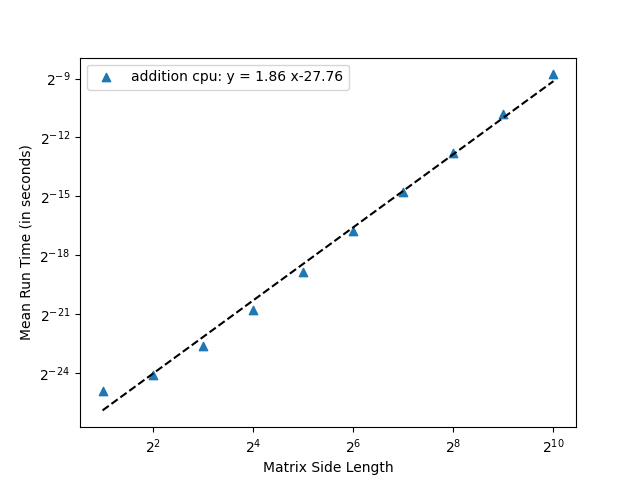
\includegraphics[width=0.5\textwidth]{SavedBenchmarksAndDiagrams/Machine 2/Addition/CPU.png}
%     \caption{CPU Addition Benchmark}
%     \label{fig:addition_cpu_bench}
% \end{wrapfigure}

\begin{figure}[ht]
    \centering
    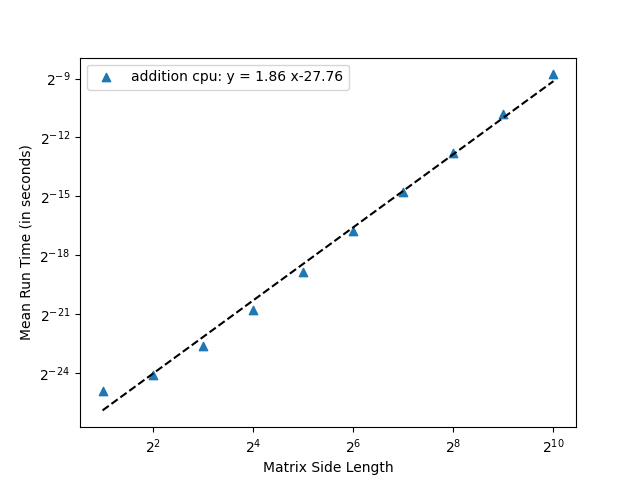
\includegraphics[width=\textwidth]{SavedBenchmarksAndDiagrams/Machine 2/Addition/CPU.png}
    \caption{CPU Addition Benchmark}
    \label{fig:enter-label}
\end{figure}

 As can be seen in figure \ref{fig:addition_cpu_bench}, our graph has a slope of 2. This is expected, since the algorithm has time complexity $O(n^2)$ and is plotted on logarithmic axes in our diagram (see sect. \ref{subsect:benchmark}).

Note that for each \texttt{element}, only 1 arithmetic operation has to be performed. The overhead of running this on GPU might outweigh the benefits of parallelization, simply because of the relatively little work each core on the GPU will have to do. Keep this in mind as we dive into the world of GPU programming.

\subsection{Addition: GPU Implementation Single Core}
The first GPU is essentially running our CPU implementation on a single core on the GPU. Again, it runs a single for-loop iterating over every element in the input matrices, adding them, and storing the result in the result matrix (see listing \ref{lst:gpu_addition_single_core}).

\begin{lstlisting}[language=C, caption={GPU addition single core}, label={lst:gpu_addition_single_core}]
__global__ void cuda_matrix_addition_single_core_kernel(
    device_matrix_t matrix_a, device_matrix_t matrix_b,
    device_matrix_t matrix_c, int size, int rows, int columns) {
    for (int i = 0; i < size; i++) {
        matrix_c[i] = matrix_a[i] + matrix_b[i];
    }
}
\end{lstlisting}

For launching kernels we wrote an algorithm runner, which can run any algorithm, which takes three matrices as parameters, as well as three integers. These integers are used for different parameters in our algorithms. For instance in addition, they are the totalsize of the matrix, the row count and the column count. The size is passed as a parameter to precompute it, instead of computing it in each kernel. It can, however, be derived from the row and column count. 

We wrote the algorithm runner because much of the code, when writing code for the GPU, is essentially "boilerplate". All addition- and multiplication algorithms requires us to allocate the matrices on the device, copy the matrices over from host to device, run the kernel, and then copy the result matrix back. This "boilerplate" code can be found in listing \ref{lst:algorithm_runner} in appendix A.

Launching a kernel requires a grid size and block size. For this implementation both are 1, since we only run code on a single core.

In benchmark (INSERT GPU VS CPU SINGLECORE BENCHMARK), it can be seen that the GPU implementation is a lot slower than the CPU implementation. '

% In fact, it seems that the launching of the kernel is very slow, since there is no real difference in running time between matrix side length $2^1$ and matrix side length $2^5$. To further substantiate this we have % TODO: INSERT CUDA_DIAGNOSTIC PART

\subsection{Addition: GPU Implementation Multi Core 1}
The following implementation will utilize the architecture of the GPU and the CUDA-specific utilities discussed previously to run the algorithm on multiple cores. Instead of calculating all $n$ elements on one kernel, we will initiate $n$ many kernels to do the job in parallel. Conceptually, the matrix is split up such that each row of the matrix is contained in its own CUDA-block. Further, each entry of a row is sent to each individual CUDA-thread of the CUDA-block. In programming terms, the i'th block and the $j^{th}$ thread will be responsible for calculating element \texttt{matrix\_c[i][j]} and this element only. 

In listing \ref{lst:gpu_addition_multi_core}, we use the blockIdx.x, blockDim.x and threadIdx.x to calculate which element this thread must work on. These values are available in any kernel, provided by the CUDA library. Note this calculation is essentially the same we used for the INDEX macro, described in section \ref{sect:datastructure}. 

\begin{lstlisting}[language=C, caption={GPU addition multi core}, label={lst:gpu_addition_multi_core}]
__global__ void cuda_matrix_addition_multi_core_kernel(
    device_matrix_t matrix_a, device_matrix_t matrix_b, 
    device_matrix_t matrix_c, 
    int size, int rows, int columns) {
    
    int index = blockIdx.x * blockDim.x + threadIdx.x;
    matrix_c[index] = matrix_a[index] + matrix_b[index];
}
\end{lstlisting}

This has one major limitation: NVIDIA only allows block sizes up to 1024, so implementation only works for matrices with a column count of up to 1024.

INSERT BENCHMARK

\subsection{Addition: GPU Implementation Multi Core 2}
We experimented with another way to utilize the CUDA-architecture, to see if it would improve our performance. This time, we would hardcode the number of threads in each block to be 16. This way, we hope to better take advantage of each multiprocessor and solve the major limitation of the previous algorithm.

Because each multiprocessor is responsible for scheduling the execution of thread-blocks, it would not make sense for each block to have 1024 threads that all have to finish before the multiprocessor can schedule a new block. Also, as discussed in \ref{background_gpu}, small blocks allow our algorithm to scale better on a plethora of devices with different SM counts.

Each block will consist of 16 by 16 threads, meaning 256 threads in total. Each grid will consist of $rows / 16$ by $columns / 16$ blocks. To allow for arbitrarily sized matrices, we also included some padding, so the actual grid size is $(rows + 15) / 16$ by $(columns + 15) / 16$. Because of the padding we also need to have a check, so we do not get out of bounds. The implementation can be seen in listing \ref{lst:gpu_addition_multi_core_2}.

\begin{lstlisting}[language=C, caption={GPU addition multi core 2}, label={lst:gpu_addition_multi_core_2}]
__global__ void cuda_matrix_addition_multi_core_kernel2(
    device_matrix_t matrix_a, device_matrix_t matrix_b,
    device_matrix_t matrix_c, 
    int size, int rows, int columns) {
    
    int i = blockIdx.x * blockDim.x + threadIdx.x;
    int j = blockIdx.y * blockDim.y + threadIdx.y;
    if (i >= rows || j >= columns) return;

    matrix_c[INDEX(i, j, columns)] =
        matrix_a[INDEX(i, j, columns)] 
            + matrix_b[INDEX(i, j, columns)];
}
\end{lstlisting}

Because of the fixed block size, this implementation also fixes the previous problem of only allowing matrices with a column count of up to 1024.

INSERT BENCHMARK

\subsection{A note about the choice of data structure}

As mentioned earlier, at the beginning of this project we used a 2D data structure. We implemented CPU addition, GPU single core addition and the first GPU multi core addition. On the GPU side it was still simply a \texttt{float *}, and we would simply flatten the two-dimensional matrix to a 1-dimensional one and send it over to the GPU. When we got the result matrix back from the GPU we would turn it back into a two-dimensional data structure. 

We suspected that this translation between the two representations might have introduced some overhead. Therefore we decided to pivot to a fully one-dimensional approach. We decided to benchmark the two data structures against each other for both the CPU and GPU. As can be seen in figure \ref{fig:1d_vs_2d_bench}, all of the algorithms run faster with the one-dimensional approach, rather than the two-dimensional one, even on the CPU. This is likely due to the fact that our CPU implementation of addition iterates over the matrix linearly, giving optimal locality in the one-dimensional approach.

\begin{figure}[ht]
    \centering
    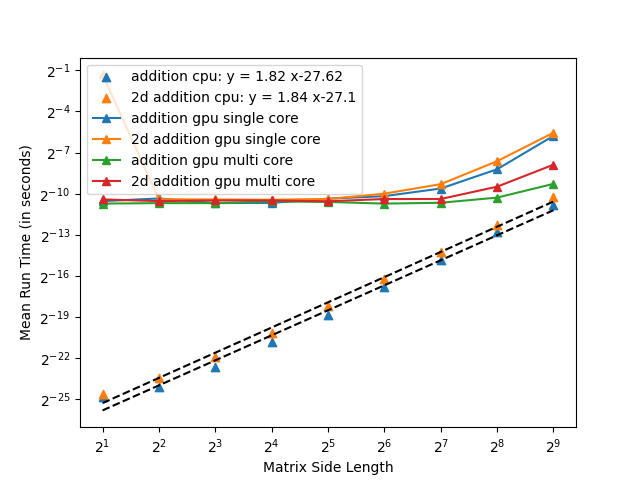
\includegraphics[width=0.65\textwidth]{SavedBenchmarksAndDiagrams/Machine 2/2D vs 1D.png}
    \caption{CPU Addition Benchmark}
    \label{fig:1d_vs_2d_bench}
\end{figure}
